\section{波动和粒子}

我们给自己设定一个任务,就是努力把事情说清楚,把事情说清楚就是使听众认同,如果没有听众就是使假想的听众——另一个自己——认同。这听起来有点分裂,但确实要求这另一个自己有一点“较真”和“不断置疑”的精神。

说服,或者使用图像,或者使用语言。而使用图像更有说服力。

图像就是图景,是Picture,但要让它动起来,这需要一点想象力。有时候我们会说动起来的图像比静止的图像更真实,这是由于人在大多数情况已经适应了动起来的图像,或赋予动起来的图像以更高的审美价值。

比如拍照,我们在任一瞬间拍下的照片都是“真实”的,但拿来看却往往惹人笑,表情的瞬间也许很丑,我们从来都没有看过小于$0.01$秒的瞬间,我们看的是“时间”的绵延,是处理过的富于动感的图像,我们是借助动感的图像建立起我们的审美,对人神情的,人动态的……审美。我们觉得眨眼很迷人,但我们觉得眼睛完全闭合的瞬间丑死了。

\begin{figure}[htbp]
\begin{center}
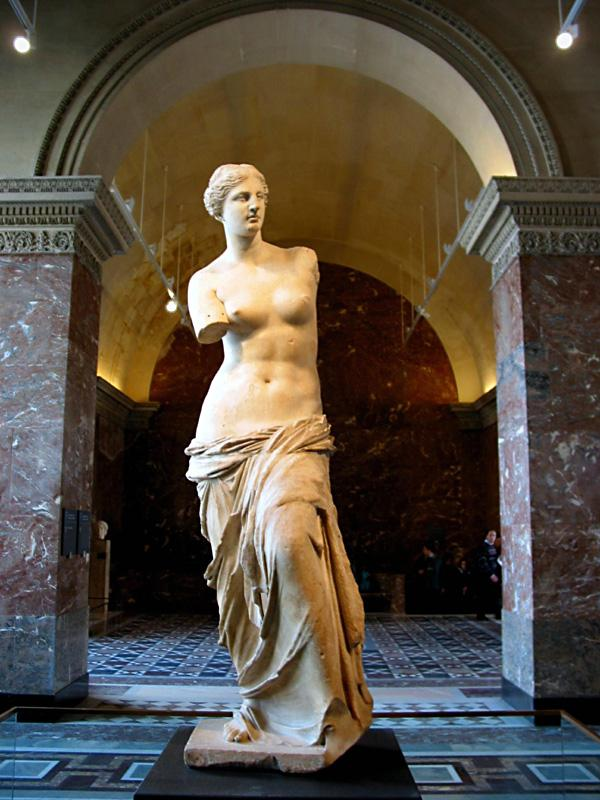
\includegraphics[width=9cm]{Duality/venus_de_milo.jpg}
\caption{米洛的维纳斯像:看起来有动感的雕像都有不符合解剖学比例的地方。}
%\label{default}
\end{center}
\end{figure}

在我们的想象中要让比如一个点动起来,一个三角形变大,旋转……是需要想象力的,而我们确实有这样的能力,有时我们在瞬间看到万丈光芒,极度具有结构特征的几何图形,色彩的斑驳变化,伴随着节奏、音乐的节奏,或我们思绪的内在节奏,在自己的脑海里轮番更替。

在这样的瞬间我们仿佛透彻了宇宙间所有的真理,但却没有合适的语言把它们描述下来,我们只能试一试,努力凭记忆把它们画下来,借着篝火,用颜料涂抹在山洞的顶上。

一些极富想象力的抽象作品。

据说这种抽象风格的绘画和极度写实的绘画同时出现。“写实”是对“可见”事物的模仿,而“抽象”是对“可以想见”事物的模仿。它们都是有力量的存在。

今天的人会设想,也许是出于交流或记录的目的,我们的祖先才开始绘画。但也有人说最早的绘画应该没有任何教育或交流的目的,它纯粹是出于精神的需要,是人灵性的发泄,是与神亲近的方式,所以它们才被创作于黑黢黢的山洞里面。

\begin{figure}[htbp]
\begin{center}
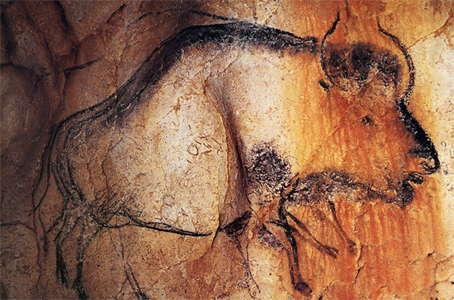
\includegraphics[width=8cm]{Duality/runningbisons.jpg}
\caption{肖维岩洞(Chauvet Cave)中的绘画已经有三万多年的历史了,几乎与人类本身的历史一样悠久,图中奔跑的野牛被表现为有很多条腿的野牛。}
%\label{default}
\end{center}
\end{figure}



\subsection{粒子的图像}

我们现在就需要通过想象而非观瞧来建立关于粒子的图像,和关于波动的图像。这是我们谈论波粒二象性的前提。

何谓粒子?

它是一个点,理想的点,只有方位,而无部分。在我的想象里它居于一个三维的空间,我可以让它上下稍微动一动,而完全不会影响其在左右方向上的位置,也不会影响其在前后方向上的位置。

假如世界只有这一个粒子,这是多么的空洞。

它可以任意地上下、左右、前后地改变位置,但对我来说是完全一样的。它都在我想象的空洞空间的中央,位置的改变无从说起。

我们必须有个参照,有了参照,我们就能说出粒子的位置了。

这个参照就是三把想象的尺子,它们互相垂直构成一个参照。或我们需要第二个点,作为原点,粒子是参照原点运动变化的。我们还需要三个箭头,标明三维空间的三个方向。

但“三”,为什么是“三”呢?

这是我们对我们所在空间的合理分类。

分类是理性的活动,是智慧的活动,谁善于分类谁就是聪明人!

“亚当证明自己是世界上第一位且最伟大的哲学家:他能根据物种的真正的本质和差异恰如其分地对它们加以区分。”

合理分类的标准是:既不重复,也不遗漏。

把我们所在的空间分解为三个不同方向是既不重复也不遗漏的。

我们也可以设想二维或一维的世界,这或者是出于限制,比如我们人类的活动就长期被限制在二维的空间上,当然是在球面上。物理学家现在也喜欢谈量子限制效应(quantum confinement effect),所谓限制就是出于某种原因,粒子(比如电子)就仅仅在二维或一维空间里运动。

想象低维空间的好处是想起来比较容易。比如落体运动,其实就是粒子在引力的作用下以越来越快的速度下落,描述这个运动只需要想象一维空间。比如炮弹的运动,就是粒子一方面以初始速度往斜刺里飞,要想飞的最远就需要以$45^o$的角度往斜刺里飞,另一方面粒子仍然受引力的作用在以越来越快的速度往地面落。

所以这是一个想象中的两个运动的叠加,先往斜刺里飞一段,再往下掉一段,然后再往斜刺里飞一段,然后再以更大速度往下掉一段。最后在我们的想象中再让这一段段锯齿缩小,让它看起来圆顺光滑一些,这就是炮弹的运动——抛物线了。

我们还可以想象很多,比如坐过山车,呼啸而下,越来越快,心悸的感觉,然后在极度的空虚中,我们向上,越来越高,在最高处,时间仿佛停止了,其实是此时速度最小,最后向下,加速,新的循环开始。

这里的窍门,是把我们自己想象成粒子,把自己的心替换为粒子的心,让我们进入粒子的世界。我们会感到有风迎面吹来,感到阻力,……

阻力是阻碍粒子运动的。我们喜欢引力,只要速度合适我们能围绕一个引力的中心(比如地球)循环往复地运动起来,一个椭圆:当我们如过山车一般冲向地球的时候,我们的速度最快,因为速度,我们从离地球最近的地方呼啸而过,然后摆脱地球,离它越来越远,向上,弯曲着向上,依靠惯性,或依靠动能($K = \frac{mv^2}{2}$)反抗地球的吸引,直到冲到离地球最远的地方,空虚地失去了太多动能,然后引力又占了上风,拉着我们加速下降,如此循环。

我们在飞,我们努力想控制飞行的轨迹,但很可惜,我们没有办法,就像梦境中的人想努力控制自己的飞行一样,徒劳和无能为力,我们在虚空中飞行,引力是唯一的外部原因,它严格地按$F = \frac{G M m}{r^2}$行为,椭圆轨道由我们的初始冲动决定,即我们在距离地球多远的地方,决定以一个什么样的速度,什么样的角度,开始运动。

(对一个二阶常微分方程$F = m a$来说,只要给定两个初始条件,初始的位置$x_0$和初始的动量$p_0$,粒子的运动就完全决定了。换句话说我们就能求解出粒子运动的轨迹。)

粒子是我们现在思维的基本单元,每个粒子都可以用质量,位置,和动量来描述。

质量就是粒子的质量。我们假设万事万物都有质量,但光子(光的粒子)除外,我们暂时先不讨论它。位置就是一个三维矢量,我们一般把它记为$\vec r$,它分解为三个固定方向上向量的叠加:

\begin{equation}
\vec r = \vec i x + \vec j y + \vec k z
\end{equation}

动量的定义是质量乘以速度,速度定义为对位置的微分:

\begin{eqnarray}
\vec v & = & \frac{d \vec r}{d t} \\
\vec p  & = & m \vec v
\end{eqnarray}

位置,速度,动量都是矢量,还有力,这给我们的想象力带来极大的挑战,为了思维的轻松,我们往往把它们想象为二维的或一维的。

粒子在三维空间里飞来飞去,但它并没有自由意志,它是由力和它的初始状态完全决定的,我们可以把粒子位置随时间变化的关系求出来。

\begin{equation*}
 \vec r(t)
\end{equation*}

粒子如$\vec r(t)$般在时间和空间里存在,$\vec r(t)$就是粒子的世界,粒子的一生,它完全由它受到的力,它的初始位置和它的动量决定。这是很宿命的世界。

如果只存在牛顿力学,我们的世界就是这样的一个世界。万事万物不过是粒子的集合,很多很多个粒子,虽然多,但它总数的过来,比如整个宇宙中质子的数目就是$10^{80}$数量级。

只要可数,我们就可对它们列方程:可数个质点,可数个力,可数个初始位置,可数个初始动量,一个非常巨大,但确实是可数个微分方程联立,虽然我们不可能对这$10^{80}$个方程求解,但它们的解是存在的,我们求不出是因为我们人自身的局限。

如此巨大的方程,在我想象的世界里是即刻被求解出来的,$10^{80}$数量级的粒子,它们冲撞,互相缠绕,各自远离,经过无限时间后又相互吸引,重新凝聚……就如一场戏剧在笛卡尔空间这个三维的舞台上出演。

每个粒子都是莎士比亚戏剧中的一个人物,各有各的命运,但这一切在戏剧开演的一瞬就已经决定,我们张大嘴巴好奇地看,假想自己进入到戏剧里,与某个粒子化为一体,或进入环绕某个粒子运行的轨道,我们有我们的自由意志,但我们就如梦境中的人一样,我们根本就无法驾驭粒子的运动,我们徒劳地想,徒劳地扭动思想的身躯,但这场戏只由力,初始位置和动量决定,我们的命运早已被安排,只是我们不知道。而我们所有的意志都是无用的,我们不受我们自己指挥。

\begin{figure}[htbp]
\begin{center}
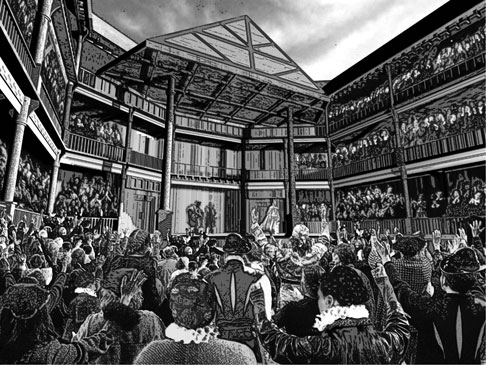
\includegraphics[width=8cm]{Duality/ShakespeareanTheater.jpg}
\caption{莎士比亚时期的舞台提供给我们想象空间和运动的原型。}
%\label{default}
\end{center}
\end{figure}

所谓粒子的图像就是粒子们在虚空中运动,它们各有各的质量,相互之间存在着万有引力。假如上帝是造物者的话,他在造物的瞬间会用他的大手抛洒出这$10^{80}$数量级的粒子,然后以他的全能使其按各自的方式具有初始位置和初始动量,然后他老人家就休息了,在异度空间翘着脚看质点们成形(pattern formation)演化。

这里虚空很重要,无虚空粒子就没有舞台。而所谓质点则是一些没有大小、形状的几何点,它们可以集中地携带一份能量和一份动量。虚空是古代原子论强调的,但他们认为原子有形状,因为古代原子论者没有发现相互作用(力),它们需要形状来解释物性。

古代原子论者还会强调有粒子的突转(swerve),这是想给它们灰暗的世界图景保留一点人性的努力,突转后来被看做是“自由意志”的体现,被挪用到基督教哲学中。引入突转纯粹是哲学的考虑或审美的原因,这在僵硬或被构建得很死的牛顿力学里是没有地位的。粒子有没有自由意志,会不会突然神经质似的蹦跶一下是微分方程($F = ma$)决定的,它告诉我们不行,就是不行!

牛顿力学关于世界的图景是缺乏解释力的,它归根到底只是一个关于机械运动的理论。原则上说由此出发可以构建一个物性的理论,甚至一个电磁学的理论,但实际上太不可行了以至于几乎没人尝试。

\subsection{波动的图像}

牛顿本人也研究光学,它认为光是由很多细小,运动速度很快的粒子组成的,这其实就是在延续古代原子论者的观点。光的粒子说可以解释光的直线传播,光的反射、折射,光可以被物体遮挡等常见的光学现象。

牛顿的粒子说是很不完备的,仅可看作是为了理解方便而做的一种权宜性假设,比如他并没有告诉我们光的粒子(光子)的质量是多少?它的能量是多少?它的动量又是多少?以及如何由这些基本的物理陈述出发,解释牛顿环的条纹间距。

仅仅说光子砸在玻璃上然后激起涟漪形成了圆环是很有想象力的猜测,但还不构成一个靠谱的理论。

一个靠谱的光学理论必须能够对最突出的光学现象做出定量的解释。就好像我们在氢原子的玻尔理论中体会到的,一个靠谱的关于原子的理论首先要能定量地解释这个领域里最独特而且也是最显著的现象,比如——里德堡公式。

\subsubsection{三棱镜分光实验}

波动图像的兴起和牛顿粒子图像在光学研究中的无能为力有关。但吊诡的是牛顿同时还是近代光学实验的先驱,他做的那些实验恰恰可以用波动说去解释。

这里我们只讨论他的三棱镜分光实验。

\begin{figure}[htbp]
\begin{center}
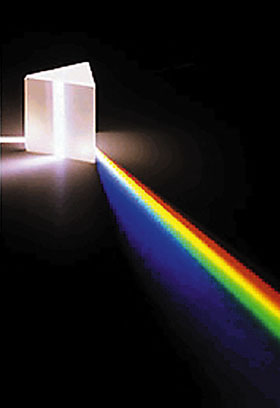
\includegraphics[width=5cm]{Duality/newtonprism.jpg}
\caption{牛顿的三棱镜实验。}
%\label{default}
\end{center}
\end{figure}

彩虹是自然界中常见的现象,又或者我们喝口水对着太阳喷一口,就可看到圆弧形的颜色分布。这些都提示我们,光,看上去很纯,但其实很复杂,也许还可以进一步分类。

牛顿就是那个对光进行分类的聪明人,他是这么做的:

在封闭的屋子里,把厚厚的窗帘稍稍拉开一条缝,使光透进来,然后拿一个玻璃做的三棱镜,玻璃的折射率比较大,它可以使光比较明显地偏离原先的运动方向。但玻璃的折射率对不同波长的光是不一样的,不同波长的光会有不同偏转的角度,不同波长对应不同颜色,一束白光于是就被分成了一系列颜色的光。

假如我们只留下一种颜色,把其他颜色挡掉,继续让光通过三棱镜,我们发现光不会再继续分解了。

在我们的视觉经验里,自然光或白光是纯净的,但现在白光是复杂的,可以被某个操作继续分解,而带颜色的光反而有可能是纯净的了,它不能被这某个操作继续分解。

\begin{table}[htdp]
\caption{可见光的波长($nm$)}
\begin{center}
\begin{tabular}{|c|c|c|c|c|c|}
\hline
   紫 & 蓝 & 绿 & 黄 & 橙 & 红 \\
   380-450 & 450-495 & 495-570 & 570-590 & 590-620 & 620-750 \\
  \hline
\end{tabular}
\end{center}
%\label{default}
\end{table}%

初看起来这有点象变戏法,但为什么我们相信科学家(但不相信魔术师)呢?

原因是科学家不隐瞒自己的发现,科学家做演示(实验其实就是一种“公开”的演示),但他会把演示的步骤一步一步告诉你,使大家都能重复。这个说法在今天有点不确切,但主要是因为科学已经发展到极其复杂和昂贵的程度,致使普通人很难重复他们的工作,但在科学家社群内,各个竞争的小组还是可以的,否则科学发现就不会得到确认,科学活动的功利价值——通过首先发现权获取名誉和利益——就无从体现。

而魔术师就不一样了,他也表演,但他不会教你,除非你付钱成为他的徒弟。

科学活动有一套规范能够认定牛顿并非是在变戏法晃点大家,否则这么反常识的结论大家是不会承认的。而今天我们讨论科学的时候也一定要记住,科学之所以可信,并不在科学方法的严谨,也不在科学家多么有良心,而全在有一套科学实作之成规,我们信赖的是制度,而非个人或具体的科学知识。但普通人在谈论科学话题的时候往往因为知识上的欠缺,就先自己矮了一头,这是不对的,我们当然需要一定的知识做基础,但我们考虑问题的焦点应该是拷问科学实作的成规,检讨其在运作中的漏洞等等。

(这里面的道理其实很简单,假想你是个总统,你需要做决策,很多方面的决策,并对这些决策负责,但显然你不可能是每一方面的专家。)

\subsubsection{水波}

牛顿关于光学的系列实验开创了物理光学,而牛顿粒子说的无所作为则给了波动说机会。

波动也是我们日常生活中常见的图像,比如:水波。

假设我们身处一个巨大的游泳池,或者有人造的海浪或者有天然的海浪(以海为池),套上游泳圈,我们会随着波浪周期性地一起一伏,这是很好玩的体验,起来到顶是波峰,而降到低是波谷,在波峰的时候,我们会看见远处某段距离外的波峰向我们移来,当我们降到谷底的时候,我们会感到波峰离我们越来越迫近,像座小山一样扑来,然后我们随着这下一个波峰的到来和救生圈一起飞快的上升,很像坐过山车,到了波峰的顶部会有空虚的感觉,然后又加速向下,如此反复。

没有水面我们就体验不到这美妙的运动,在每个波峰来临的时候,我们都感到它巨大的力量,它狠狠地把我们从谷底掀起来,往上扔,波峰越高,我们越体验到它巨大的力量。我们无时不刻、处处体验到波的能量,当我们冲到波峰的顶部的时候我们有很大的势能,势就是“位置的优越”,因为我居于此位置,我可以把这位置的好处转化为运动的动能去冲,而当我们居于波谷的时候,我们其实是处于另一个波峰,因为水波的弯曲,水波整体的挤压,我们仍然会居“位置的优越”,或换句话说,我们仍有一个大的势能……

波的能量正比于振幅的平方($\propto A^2$),水波的能量分布在整个水面,波传播到哪里,波的能量就到哪里,我们套上救生圈就可以体验到这种能量。

波是整体的运动,当我们研究水波的时候,能量并非集中在某一点,它是能量的分布,“均匀”地分布在整个波动着的水面。此时虚空的概念就多余了,空荡荡的舞台可以让莎士比亚戏剧中的人物一个个登场,但水波必须要有个游泳池,里面装满水,水波存在于水波的表面上。

在水面上,每一点都随着水波在波动,我们如果一个一个位置地去描述水波的运动可要累死了,因为位置是不可数的(innumerable),我们没有办法用$1, 2, 3, ...$的方式遍历水面上的每一个位置。这是和我们研究牛顿粒子世界的一大区别,在那个世界里,有$10^{80}$数量级个粒子,虽然很多,但到底可数,可以用$1, 2, 3, ...$的方式穷尽。

这里我们必须说$1, 2, 3, ...$的方式其实是个很强大的方式,如果你不限定时间的话,我们可以穷尽无穷多个粒子。这个无穷有专门的名字,叫:“阿列夫零”,即最低阶的无穷多,或可数的无穷多,即用$1,2,3...$数数的方式可以穷尽的无穷多。

\subsubsection{无穷多的自由度}

由此我们已经进入了场论的研究领域,所谓场论就是研究无穷多自由度的运动。场就是物理量随时间、空间的分布,比如电场$E(x,t)$,空间上的每个点$x$都有自己的场,不同位置的场如$E(x_1)$和$E(x_2)$的取值是独立的。

$E(x_1)$和$E(x_2)$是独立的自由度,或每个不同的$x$对应的$E(x)$都是一个独立的自由度,考虑到在空间里有无穷多个$x$,我们这里就有无穷多的自由度。

(自由度就是描述一个物理系统所需要的独立变量的个数,比如对自由落体,只需要一个,即位置。)

假设我们讨论一个经典的场论。我们应如何研究波动呢?

一种方法是把它离散化,因为处处皆在的连续太难想象了。我把它们想象成为一个弹簧床垫,在场里面做想象的切割,每一个小方块,或每一个三角形,六角形,收缩成为一个质点,每个质点的质量将等于面积乘以密度,然后我在想象中让每一个质点按照某种结构相连,用假想的弹簧相连,如果你不想让你的场破碎的话,你就必须用弹簧把它们编织起来。

此时上帝变成了一个编织弹簧床垫的工人,弹簧各有各的弹性系数,它们可用弹性模量来表示。离散模型的好处是好想。一个离散的模型又部分地回到了粒子的图像,但粒子是被固定在各自平衡位置附近的,它们被弹簧束缚住,不能自由地在虚空中跑来跑去。

波的能量现在体现为所有质点的能量和,而每一个质点又由动能和势能两部分组成,很多细小的$\frac{1}{2} m v^2$和$\frac{1}{2}k x^2$之和,然后利用密度,弹性模量等概念再重新把这些关系表示为连续的情形。这时我们会得到一个用连续的场$\varphi(x,t)$表示的动能和势能。

我们使用一套由牛顿力学发展出的技巧(相当于是某种数学变换),我们不考虑力,转而考虑拉氏量$L = T - V$,它的定义是动能减去势能,由拉氏量出发我们利用一个变分求极值条件,就可以得到波动方程。波动方程和我们利用偏微分方程技巧求得的形式是相同的。它的解却可以是自由的,即波可以在弹簧床垫里自由地传播,并不衰减。

这是一个很漂亮的结果,如果你把“弹簧床垫”看做是个粒子的世界的话,这里的粒子是“固定”不动的,它们只能在各自位置的附近做微小的振动,但这些振动由于弹簧的耦合,却可把一个局部的振动向各个方向传播出去,传播给其他位置上的粒子。整体看就是一个波动在自由地传播,所谓自由指的是波动在传播的过程中并不损失能量,而且波动确实是可以传播到弹簧床垫的任意部分的。

\subsubsection{波的干涉}

两列波相遇,会发生干涉现象。这也是我们极熟悉的自然现象。

比如在夏日的傍晚,我们来到一个池塘边,有轻风吹过水面,池塘里泛起一阵涟漪,此时追踪波的运动,观察它,假如波撞在一根芦苇上,我们会发现水波似乎以芦苇为中心形成了一个新的波,你如果仔细看,还会发现波每碰到一个细小的障碍物,都会以此为中心形成一个新的波,以同心圆的形状向外扩散。

波动运行中的每一个点都可看做是一个新的波源,而波动整体的效果就是这无数波源扰动的波动的叠加。这就是惠更斯原理。

这么说很有美感,只是具体计算的时候会很麻烦。但假如波动撞到某面墙上,我们在这墙上只开两个小孔,这个运算就会变得简单。我们只需要计算两列波的叠加,这两列波其实是源自同一个波的,是我们把它们的兄弟姐妹们都挡住了。

如前所述,波动可以看做是相位的奔跑,相位是$k x - \omega t$,假如我们考虑某一时刻波动的情况,即$t$是固定的,我们需要看的是$k x$。

现在一列波由A出发按照某个路径(Path A)跑了$x_A$距离,相位是$k x_A$,而另一列波由B出发按照某个路径(Path B)跑了$x_B$距离,相位是$k x_B$,假设这两列波最终在C相遇。

如果相位差$k (x_A - x_B)$正好是$2 \pi$的整数倍,意味着两列波是同步的,振幅会变为$2A$,而波的强度则会正比于$4A^2$。

但假如相位差$k (x_A - x_B)$正好是$\pi$的奇数倍,则意味着当一列波位于波峰时,另一列波必位于波谷,它们总是相消的,振幅会变为$0$,波的强度也只能是0了,这是无法再弱的情况了。

当然还有居于二者之间的情况,但我们不妨把最强和最弱(0)当做标志。

\begin{figure}[htbp]
\begin{center}
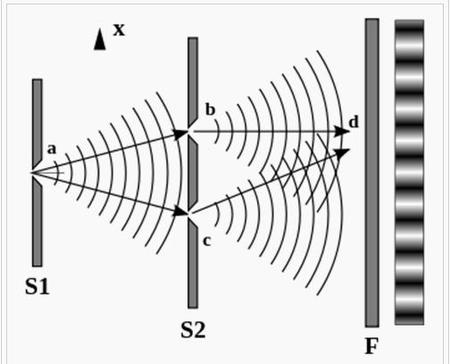
\includegraphics[width=8cm]{Duality/doubleslit.jpg}
\caption{双缝实验示意图。}
%\label{default}
\end{center}
\end{figure}


这就是著名的双缝实验,我们将会在双缝的对面观察到一系列振动“最强、最弱、最强、最弱……”的条纹分布。

对水波而言,我们是能直接看到这种现象的,所谓水波涟漪。就是这种波峰、波谷错综相杂的条纹镶嵌。

光的干涉要难些,首先对光源有要求,我们必须用特定波长的光源,而且光源要稳定,行话叫相干光;另外由于光的波长本来就很短,这需要我们专门设计实验才能观察到干涉现象。

~

光的干涉现象用波动图像很容易解释,而这仅仅是个开始,还有衍射现象,艾里斑等。衍射光栅因为对分辨不同频率/波长的光具有特别强的分辨本领成为测量光谱现象强大的工具。

物理光学就是波动光学,它很快超越几何光学成为光学研究的主流。比如我们可以用衍射光栅测量氢原子的光谱,类似地还有钠原子光谱,我们只要在炙热的火焰里放进某种元素的金属丝,我们就可以研究这种元素的光谱了。

到19世纪,光的波动说开始全面占上风。等到赫兹做实验证明电磁波也是波动,并且如光波一样有干涉、衍射等现象,物理学家普遍相信光波就是一种电磁波,光的粒子说就正式被扫进了历史的故纸堆。(就像我们现在说到以太或燃素的感觉一样)

但情况在一点点的起变化。

\subsection{黑体辐射}

19世纪末,随着工业的进步,人们开始用衍射光栅去研究黑体辐射。所谓黑体就是一个大空腔,这个空腔包纳着一个大空间,这个空间就是电磁场的海洋,各种电磁波在空腔里碰撞奔腾着,就好像是个电磁波的冲浪游乐场。空腔(把它想象为太上老君炼丹的炉子)的温度是可以调节的,电磁辐射场与空腔达成了热平衡,所谓热平衡是个与材质无关的事情,这很平等,铁的$300^o$和陶瓷的$300^o$是一样的,它们都能和$300^o$的电磁辐射场达到热平衡。

我们还记得热交换的几种途径:传导、对流和辐射。这个辐射就是电磁辐射,太阳离我们很远,中间又没有导热的介质,传导和对流都无从谈起,靠的就是辐射。所以我们说辐射、热辐射,还是电磁辐射讲的都是一个东西。

我们可以在想象中把电磁辐射场的一部分画个范围,其内是个物体,这个物体——其实就是电磁辐射场——与腔体通过辐射达成热平衡,假如腔体的温度是$T$的话,那么电磁辐射场也处在温度$T$。

现在温度进来了。

在统计物理的框架内,温度和无规则的热运动有关,无规则代表着信息的缺失,我们没法知道系统内每一个质点的运动,但我们知道它们作为整体的统计规律,这个规律说,质点具有动能$K$的几率正比于玻尔兹曼因子$e^{-\frac{K}{kT}}$。这个概念我们可以推广运用到黑体辐射中。

所谓黑体辐射就是很多电磁波的振动,很多振动的模式,它们的能量正比于电场强度的平方,也正比于磁场强度的平方,而现在电场和磁场就相当于质点的动能$K$。

我们不进入计算的细节,只是声明统计物理现在就能排上用场了,我们有很多振动的模式,每个振动模式用不同的波矢$\vec k$表示,很多波矢,每个波矢对应的振动都有能量,我们希望把这些能量都加起来,我们现在并不知道每个振动的能量,我们求热力学平均,再把它们加起来,并把能量的密度$u_T(\nu)$用波长或频率表示出来。

\begin{equation}
u_T(\nu) = \frac{ 8 \pi }{ c^3 } \nu^2 k_B T
\end{equation}

这是一个很漂亮的计算,就一个毛病,计算出来的能量密度对短波长(或高频率,所谓紫外)是发散的,即$\nu \to \infty$时,$u_T(\nu) \to \infty$。这导致了一个荒唐的结果,即每单位空间我们都有无穷多的能量在等着我们。而且理论计算出来的能量密度随波长的分布与实际实验测量的结果也不匹配。

1900年,普朗克利用内插法凑出了一个黑体辐射的能量密度公式,与实验数据符合的很好:

\begin{equation}
u_T (\nu )  = \frac{ 8 \pi h \nu^3  }{ c^3 } \cdot  \frac{1 }{ e^{ \frac{ h \nu }{ k_B T } }  - 1 }
\end{equation}

这个公式叫普朗克公式,它是凑出来的,我们还需要把它推导出来。但考虑到三维太复杂了,我们先考虑一维,然后由一维的结果推广。

首先对电磁波而言,每个波矢$k$都有两个独立的振动模式,比如一个是$x$线偏振光,另一个模式就是$y$偏振光。其次对大小为$L$的一维空间而言,电磁波存在于这样一个空间里需要满足一定的边界条件,比如在边界处某个方向的分量为0等等。这要求波矢满足这样的关系:

\begin{equation}
k L = n \pi
\end{equation}

这里$n = 1, 2, ...$,可见并不是一个$k$允许,而是一系列的$k$都满足边界条件和波动方程,所以我们考虑的空间里是很多不同波矢电磁波的叠加。

把这个结果推广到三维:

\begin{equation}
\frac{1}{8} \cdot 2 \cdot \frac{4 \pi k^3}{3} V = N \pi^3
\end{equation}

针对这个公式做一些说明:

\begin{enumerate}
\item 

因子$\frac{4 \pi k^3}{3}$对应的是波矢小于等于$k$包围起来的波矢空间的体积;

\item

因子$\frac{1}{8}$表示我们这里的求和是只针对$k_x >0, k_y > 0, k_z >0 $进行的,对应是波矢空间里的$\frac{1}{8}$体积;

\item 

因子$2$指的是对每个波矢,有两个独立的振动模式;

\item

V是电磁波所在空间的体积;

\item

$N$代表波矢小于等于$k$时系统允许的独立振动模式的个数;

\item

$\pi^3$,因为现在是三维了,波矢空间的体积乘以空间的体积对应的应该是$\pi^3$。

\end{enumerate}

黑体辐射能量密度$u_T(\nu)$是单位体积内处于频率由$\nu $到$\nu + d\nu $的电磁波的能量,当然是热力学平均意义下的能量。

现在首先要问单位体积内处于频率由$\nu $到$\nu + d\nu $的独立的电磁振荡的数目有多少,我们管它叫“态密度”(Density of states),写成数学的式子就是:

\begin{equation}
\frac{1}{V} \frac{d N (\nu)}{d \nu}
\end{equation}

首先由$\frac{1}{8} \cdot 2 \cdot \frac{4 \pi k^3}{3} V = N \pi^3$,我们可求出$N(k)$,

\begin{equation}
\frac{N(k )}{ V } = \frac{ k^3 }{3 \pi^2}
\end{equation}

然后根据$k = \frac{2 \pi }{ \lambda}  = \frac{2 \pi \nu}{c}$,把$N(k)$变换为$N(\nu )$:

\begin{equation}
\frac{N(\nu)  }{ V } = \frac{ 8 \pi }{ 3 } \frac{ \nu^3  } { c^3 }
\end{equation}

现在态密度$g (\nu)$是:

\begin{equation}
g(\nu) = \frac{1}{V} \frac{d N (\nu)}{d \nu} = \frac{8 \pi \nu^2 }{ c^3 }
\end{equation}

现在黑体辐射的能量密度可表示为:

\begin{equation}
u_T (\nu) = g (\nu) \left\langle \epsilon (\nu)  \right\rangle_T
\end{equation}

这里$\left\langle \epsilon (\nu)  \right\rangle_T$表示对振荡频率为$\nu$的电磁波能量的热力学平均。

如果使用经典的统计物理,我们需要做的就是对电磁波的能量$ \frac{\epsilon_0}{2} E^2 + \frac{1}{2 \mu_0} B^2 $进行热力学平均,计算结果为$k_B T$,于是我们得到了先前的那个会发生紫外发散的能量密度。

\begin{equation}
u_T(\nu) = \frac{ 8 \pi }{ c^3 } \nu^2 k_B T
\end{equation}

这个公式最早是由瑞利和金斯计算出来的,因此也叫瑞利-金斯公式。

~

普朗克面对的就是这样一个问题。他并没有直接假设电磁波本身是量子化的,他假设的是电磁波与物质发生能量交换时,必须以一份一份的方式进行,一份就是一个量子(quanta),大小是:

\begin{equation*}
h \nu
\end{equation*}

这里$h = 6.626 \times 10^{-34 }$焦耳·秒,叫做普朗克常数。现在频率为$\nu$的电磁波按普朗克的假设就是它可以用$n = 0 , 1, 2, ...$的整数份额与物质交换能量。

而以我们现在的观念则说电磁辐射本身是量子化的,对频率为$\nu$的振荡模式,它可能存在1个激发,也可能是2个激发……,当然也可以是0个激发,对应的就是没有一个$h \nu$光子的状态。

现在我们可以按照统计物理的基本法则计算$\left\langle \epsilon (\nu)  \right\rangle_T$:

\begin{eqnarray*}
\left\langle \epsilon (\nu)  \right\rangle_T &=& \frac{ \sum\limits_{n=0}^{\infty} n h \nu e^{- \beta n h \nu } }{ \sum\limits_{n=0}^{\infty} e^{- \beta n h \nu  } } =  - \frac{\partial }{\partial \beta } \ln \sum\limits_0^{\infty} e^{-\beta n h \nu } \\
{} &=& - \frac{\partial }{\partial \beta } \ln \frac{1}{ 1- e^{- \beta h \nu} } = \frac{\partial }{\partial \beta} \ln \left( 1 - e^{- \beta h \nu} \right)
\end{eqnarray*}

这里$\beta = \frac{1}{k_B T}$,所以:

\begin{equation*}
\left\langle \epsilon (\nu)  \right\rangle_T = \frac{ h \nu e^{- \beta h \nu } }{1 - e^{ - \beta h \nu }} = \frac{ h \nu  }{e^{\beta h \nu} - 1 }
\end{equation*}

最终我们得到了普朗克公式:

\begin{equation}
u_T (\nu )  = \frac{ 8 \pi h \nu^3  }{ c^3 } \cdot  \frac{1 }{ e^{ \frac{ h \nu }{ k_B T } }  - 1 }
\end{equation}

在黑体辐射实验之前光的波动说可谓是牢固地竖立起来了,但普朗克的量子假说打开了一个缺口,这之后的光电效应、康普顿散射等实验都更进一步说明光在这些实验里必须被理解为粒子才可以获得一种简单的解释。

\subsubsection{维恩位移定律}

热辐射即固体、液体或气体由于自身温度($T$)而释放的辐射。用三棱镜使热辐射折射,不同波长的光会被三棱镜折射到不同的方向上,测量不同方向上的光强分布,我们得到连续谱,即一个强度随波长连续变化的分布。

温度低于500摄氏度时,大部分热辐射能量在红外波长的区域。随着温度的升高,辐射能量的主要部分逐渐向短波高频端移动,移动到可见光,紫外光等等。

\begin{figure}[htbp]
\begin{center}
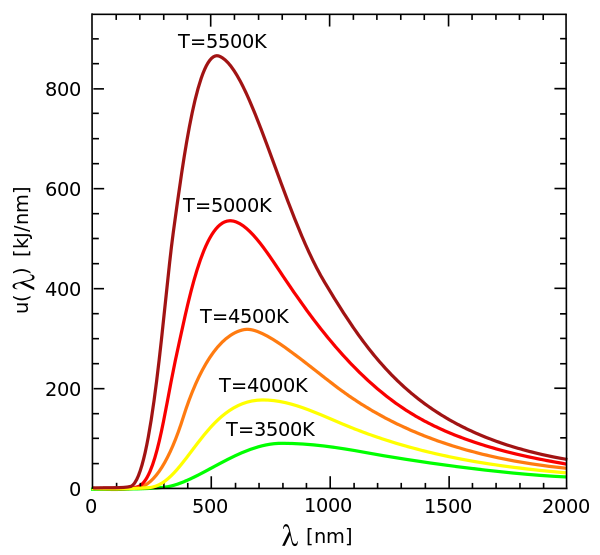
\includegraphics[width=10cm]{Duality/Wiens_law.png}
\caption{维恩位移定律。}
%\label{default}
\end{center}
\end{figure}

看来热辐射的主要部分的波长和温度是成反比的,这就是维恩位移定律(Wien's displacement law):

\begin{center}
$\lambda_{max} T = 2.898 \times 10^{-3 }$米·开尔文
\end{center}

这里$\lambda_{max}$是使谱分布$u_T(\lambda)$取最大值的波长。

这个现象本身是很常见的,比如我们在看电影《大闹天宫》的时候,太上老君把孙悟空扔进炼丹炉里烧,炼丹炉除一个开口外都是封闭的,而那个开口就是黑体,随着炉子里面的温度逐渐升高,窗口会显现不同的颜色,按照波长由长到短,或频率由低到高的次序依次出现,“红橙黄绿青蓝紫”。

用这个方法我们可以确定远方恒星的温度,比如一颗黄星的表面温度就比一颗红星的表面温度高。

\subsubsection{斯特番-玻尔兹曼定律}

物体的温度越高,发射的总能量就越多,这就是斯特番-玻尔兹曼定律(Stefan and Boltzman's law):

\begin{equation}
R(T) = \sigma T^4
\end{equation}

这里$R(T)$是辐射本领,被定义为单位表面积物体向外辐射出的功率。

\begin{equation}
\sigma = 5.67 \times 10^{-8} J s^{-1} m^{-2} K^{-4}
\end{equation}

叫做斯特番-玻尔兹曼常数。

~

我们现在可以来做一个练习:

假设太阳、地球、火星、金星都可看作是绝对黑体,利用斯特藩-玻尔兹曼定律,估算金星、地球和火星的表面温度,这给出了一个讨论温室效应的定量框架。

太阳半径: $R_S  = 6.96 \times 10^5 km$

太阳表面温度: $T_S  = 5780K$

水星距离太阳的距离是0.39AU,火星距离太阳的距离是1.52AU (1AU就是地球到太阳的距离,$1AU = 1.496 \times 10^8 km$)

根据斯特番-玻尔兹曼定律,太阳的总辐射功率为:

\begin{equation*}
P = \sigma T^4 4 \pi R_S^2
\end{equation*}

其中只有一部分会照在“地球”, 比例是: 

\begin{equation*}
\frac{\pi R_E^2}{4 \pi D^2}= \frac{R_E^2}{4 D^2}
\end{equation*}

这里$D$是地球到太阳的距离(地心到日心)。

假设地球表面温度是$T_E$,地球向外辐射的功率是: 

\begin{equation*}
\sigma T_E^4 4 \pi R_E^2
\end{equation*}

当这个辐射功率和吸收功率相等时,可估算出地球表面的温度。

\begin{equation*}
\sigma T^4 4 \pi R_S^2 \cdot \frac{R_E^2}{4 D^2} = \sigma T_E^4 4 \pi R_E^2
\end{equation*}

解出:

\begin{equation*}
T_E = T \sqrt{\frac{R_S}{2D}} = 278.77 K
\end{equation*}

这个温度与地球半径($R_E$)无关。更多结果见下表:

\begin{center}
\begin{tabular}{|l|l|l|l|l|}
  \hline
  % after \\: \hline or \cline{col1-col2} \cline{col3-col4} ...
  {} & 水星 & 金星 & 地球 & 火星 \\
  距离(AU) & 0.39 & 0.73 & 1 & 1.52 \\
  温度(K) & 446 & 326 & 279 & 226 \\
  温度(${}^oC$) & 173 & 53 & 6 & -47 \\
  \hline
\end{tabular}
\end{center}

碳基生命是发生在液态水的环境里的,而水在$0 - 100 {}^o C$保持液态,我们验证了地球确实是太阳系里最适合生命存在的星球。

%%
~

我们现在已经基本明了粒子的图像与波动的图像了。

那它们为啥不兼容呢?

从概念的角度,二者都是理想的模型,粒子要求“点”,能量和动量都被集中地携带,在虚空中穿行。而波动是运动的整体状态,需要一个介质,或像电磁波那样,电磁场本身就是实实在在的物理量,它们在时空中有个分布,波动作为一种整体的运动,能量正比于振幅的平方,充满并且连续地分布在整个介质或场里面。

场的概念比介质的概念更根本,经典物理里强调介质,无非是给出了一种使“场”得以现身的结构,一旦我们写出了场的拉氏量,场就已经数学化了,有了描述场的数学式子,我们要介质何用呢?

对电磁场的研究,我们是先得到场的陈述的,但历史上物理学家对这一数学陈述并不满意,他们试图找出电磁场的介质——以太——其实就是想构造出一种使电磁场得以呈现的机械模型。但电磁场太复杂了,物理学家们一直没成功。到了20世纪,物理学家很快就被接踵而来的新问题吸引,忙别的事情去了。

有一种克服危机的方法就是制造出更紧迫的危机,使矛盾在更高水平和更激烈的程度上爆发,具体到这里,寻找以太导致了相对论的发现,而相对论一旦被大家接受,寻找以太这个任务就不存在了。

\subsection{像波一样的粒子}

我们把Duality翻译成“二像性”,所谓像就是“like”,最有名的二像就是“波粒二像性”,字面的意思就是既像粒子又像波,或有时候像粒子有时候像波。

粒子和波如前所述是两幅图像。所谓像波,就是“wave like”,像粒子,就是“particle like”,这是个构词的游戏,我们可以说“wave like particle”,“像波一样的粒子”,或“particle like wave”,“像粒子一样的波”。

\subsubsection{电子的发现}

在历史上“波动”和“粒子”是两个相互竞争的图像,比如19世纪末,标准的科学问题是“阴极射线是一种粒子还是一种波动?”

在这类争论中,科学家们就像是在搞选举,分裂为两个阵营,以对阴极射线的争论为例,大多数德国科学家认为阴极射线是波动,而大多数英国科学家则认为阴极射线是粒子。

双方都拼命找有利于自己的证据,比如有人用集电器(法拉第笼)收集阴极射线,发现阴极射线是带负电的,由此猜测阴极射线是一种带负电的微小粒子(电的“原子”)。

对立的阵营于是就给阴极射线管加上磁场,然后论证说如果阴极射线是个粒子的话,那它应该在磁场中发生偏转,但阴极射线却没有偏转。这是波动说给粒子说的一个强有力的阻击,但显然没发生波普尔所说的证伪。

这里存在着一个问题,即实验也是可以改进的,否定性结论也和实验的方案、实验的精度有关。比如阴极射线在磁场中是应该发生偏转的,但由于实验条件的限制,比如真空度,比如磁场的绝对强度等等,德国科学家就是没有发现阴极射线能够在磁场中发生偏转。可以想象德国科学家做出了这个否定性结果很Happy,因为缺乏对粒子说的信仰,他们没有进一步改进实验的动力。

回到当时的历史情境,主张波动说意味着你必须把阴极射线看做是某种符合电磁辐射方程的电磁场,你能够通过计算解释实验中的主要现象,又或者你能够证明把阴极射线看做是一种带电粒子,将完全不能解释实验现象,或将导致与实验相反的结论。

电磁波还是带电粒子?这意味着两套方程,两种数学操作的手续,它们吃进一些数据,然后再吐出一些数据,吃进的数据是由实验来的,而吐出的数据也是要和实验比照的。如果我们采用了一套手续,就意味着我没法同时采用另一套手续。

我们讲“波动和粒子是两幅不相容的图像”,我们的意思是:它们是互相竞争、互相替代的两种理论近似(Approach)。而这两种近似又确实是以“波”和“粒子”两种图像为核心构建的。

所谓波就是充盈于整个空间的某种(物理)量的分布,比如电场和磁场,我们可以直接测空间中电场和磁场的强度,电场和磁场的强度又对应能量,因为电磁场是充盈于整个空间的,我们可以在想象中划定一块体积,能量正比于体积,单位体积电磁场的能量就是电磁场的能量密度:

\begin{equation}
\rho(\omega) = \frac{\epsilon_0 E^2(\omega)}{2} + \frac{B^2(\omega)}{2 \mu_0}
\end{equation}

这里我们把电磁场的能量密度$\rho(\omega) $表示为和频率($\omega$)有关的形式,我们在想象中对电磁场进行分类,按照不同振动的频率分类,然后再把它们加起来。

所谓粒子,就是集中地携带一份动量和能量,假如不考虑相对论的话,能量可以写为:$T + V$,动量可以写为:$p = mv$。粒子的运动满足牛顿方程。

比如带电粒子在磁场中运动,它会受到洛伦兹力$F$的影响,洛伦兹力的大小是$q v B$,这里$q$是带电粒子携带的电量,$v$是带电粒子运动的速度,$B$是磁场强度。洛伦兹力与带电粒子运动的方向垂直,如果粒子带正电的话,粒子速度$\vec v$,磁场$\vec B$和洛伦兹力$\vec F$正好构成一个右手法则

\begin{equation}
\vec F = q \vec v \times \vec B
\end{equation}

否则,如果粒子带负电,将构成一个左手法则。

引力是非常弱的,我们总可以忽略,在粒子图像下,我们就是要对粒子的受力进行分析,然后求解牛顿方程。而现在力的方向和运动的方向垂直,这符合做匀速圆周运动的条件。假设粒子做匀速圆周运动,其加速度是:

\begin{equation}
a = \frac{v^2 }{R }
\end{equation}

而向心力就是:

\begin{equation}
m \frac{v^2}{R} = q v B,
\end{equation}

即洛伦兹力正好提供了这个向心力。解出半径$R$:

\begin{equation}
R = \frac{mv}{qB}
\end{equation}

如果磁场不够强的话,半径$R$会很大,带电粒子以半径$R$做圆周运动,如果我们只跟踪粒子有限距离的话,粒子因洛伦兹力而导致的偏转是很小很小的。

真空技术和磁场是制约实验的主要因素,“真空”是对密闭的管子反复抽气制备的,这首先不是严格的真空,其次如果真空管越细小的话,成本会比较低。同样,基于成本的考虑,磁场强度也不会无限制地大。这是为什么德国科学家没有观察到阴极射线在磁场中偏转的原因。

现在需要一位信仰粒子说,坚持理想的人来拯救粒子。这是通过精巧地设计实验达成的。设计实验的人叫J J 汤姆逊,虽然是卡文迪什实验室的主任,但当时实验室的经费很少,J J也用不起大磁铁,磁场比较弱,磁场区域比较小……,这就是实验的基本限制。

\begin{figure}[htbp]
\begin{center}
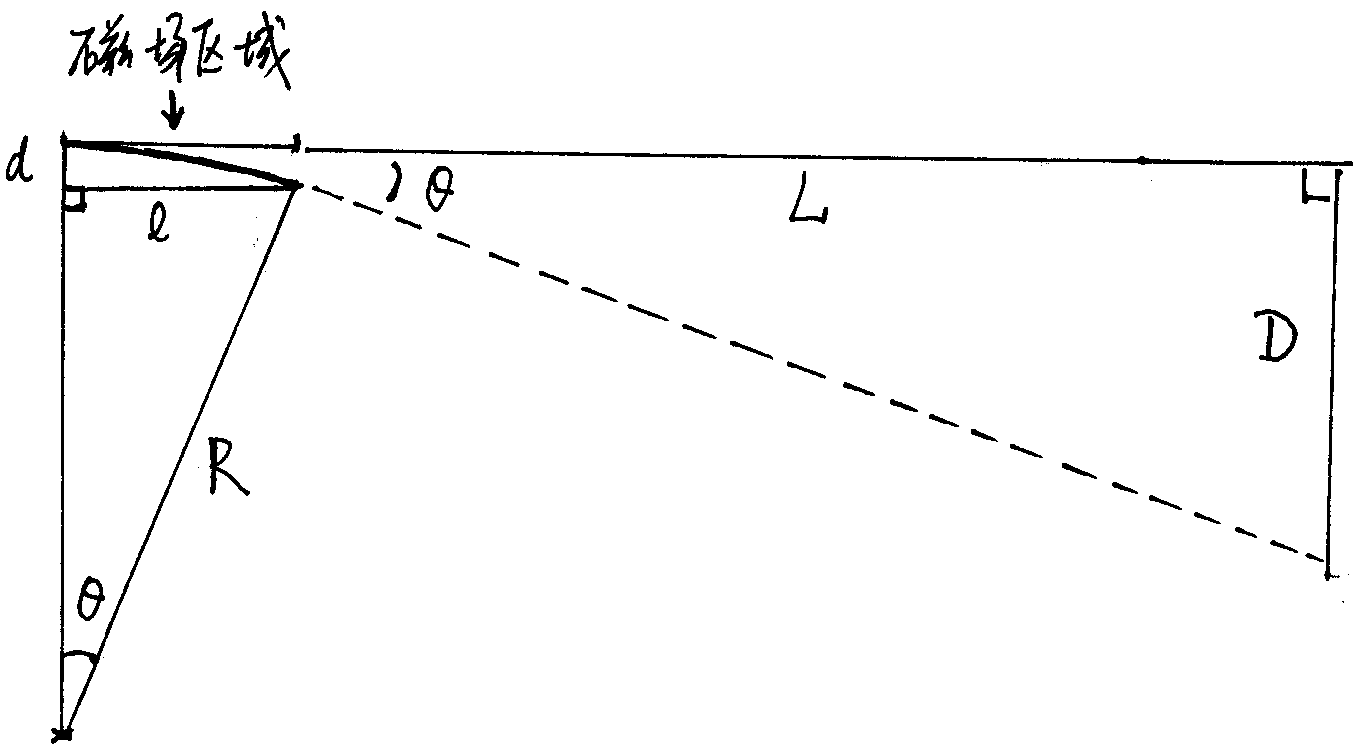
\includegraphics[width=8cm]{Duality/jjthompson.png}
\caption{汤姆逊实验。}
%\label{default}
\end{center}
\end{figure}

J J的方案是把阴极射线放出来,在经历了一个磁场区域后,再让它自由地飞一段,飞一段比较长的距离,这样偏转就会被放大。假设偏转角是$\theta$,阴极射线在水平方向上飞了距离$L$,最终在竖直方向的偏转是$D$,那么$D \approx L \theta$,即$L$越长,我们就越容易观察到偏转。

阴极射线发生偏转是因为它曾在磁场区域中运行过一段距离,假设这个距离是$l$,在这段距离里阴极射线会因磁场的存在,因洛伦兹力而偏转,偏转角度$\theta$满足如下关系:

\begin{equation}
R \sin \theta \approx R \theta = l 
\end{equation}

阴极射线在磁场里运行的时候也会有个偏转,记为$d$,这个偏转很小,很难被直接测量。但假如有这个$d$的话,线段$R - d$,$l$,$R$将构成一个直角三角形,因此有关系:

\begin{equation*}
(R-d)^2 + l^2 = R^2
\end{equation*}

化简后,可以求出:$R = \frac{l^2}{2 d}$,于是$\sin \theta$可以表示为:

\begin{equation}
\sin \theta = \frac{l}{R} = \frac{2d}{l}
\end{equation}

由于$\theta$很小,$\theta \approx \frac{2 d}{l}$。代入$D \approx L \theta$,$D \approx L \frac{2d}{l} $,求出:

\begin{equation}
 d = \frac{D l}{2 L}
\end{equation}

因此:

\begin{equation}
R = \frac{L l }{D }
\end{equation}

我们可以代入当年J J的数据来说明这个实验会碰到的困难。

在磁场区域中阴极射线飞了$ l = 0.05  $米,飞出磁场后阴极射线又继续飞了$ L = 1.1 $米,最终阴极射线在竖直方向上偏转了$ D = 0.07 $米。

由此我们可以估算:$d = \frac{ 0.07 \times 0.05  }{ 2 \times 1.1} = 0.0015 $米,即1.5毫米,确实很小,考虑到阴极射线本身撞在玻璃上会形成一个有限大小的光斑,这个偏转实际上是无法被测量的。

阴极射线在磁场中运动的半径是:$R = \frac{ 1.1 \times 0.05 }{ 0.07 } \approx 0.79$米,即将近1米,相比于$l = 0.05 $米(5厘米)或$D = 0.07$米(7厘米),确实很小。

但现在还有速度$v$不知道,如果假设阴极射线是个粒子的话,那它就可以以一个有限的速度$v$运动,为了把这个$v$表示出来,J J又使用了一个技巧,即加上一个竖直方向的电场,使带电粒子受一个与洛伦兹力正好相反的静电力,这时两个力就抵消了,偏转$D$将归零。

列出力的平衡方程:

\begin{equation}
q E = q v B
\end{equation}

因此:

\begin{equation}
v = \frac{E}{B}
\end{equation}

我们还是用J J当年的数据,电场强度$E = 1.0 \times 10^4 $牛/库,$B = 3.6 \times 10^{-4}$ 牛/安·米。

求出$v \approx 2.78 \times 10^7 $米/秒,将将是光速的十分之一,我们这里忽略相对论效应是安全的。

最终我们可求出:

\begin{equation}
\frac{m }{q } = \frac{B^2}{ E }  \cdot \frac{L l }{D}
\end{equation}

代入J J当年的数据,我们求出:

\begin{center}
$\frac{m }{q  } \approx  1.0 \times 10^{-11} $千克/库。
\end{center}

这个比值叫质量电荷比(Mass-to-charge ratio),但现在我们多用其倒数,即电荷质量比(charge-to-mass ratio),2010年CODATA推荐的数值是:

\begin{equation}
\frac{e}{m_e} = (1.758820088 \pm 39) \times 10^{11} C/kg
\end{equation}

J J 汤姆逊的实验是对粒子说的一大推动,自此之后大家就都倾向于认为在物质中存在着带负电的基本单元——电子(electron),我们把电子的质量记为$m_e$,把电子的电荷记为$e$(但我们需要记住电子所带电荷为负)

\subsubsection{油滴实验}

在汤姆逊实验之后不久,密立根又做了个油滴实验(Oil drop experiment),他把油滴通过小喷嘴喷进一个均匀电场里,在这个过程中,油滴会带上电,而电场的选择会给带电油滴一个向上的力,这个向上的力有可能与油滴本身的重力相互抵消。(必须提醒的是我们这里对实验的讨论是大大简化的。)通过显微镜我们可以找到那些“静止”的油滴,然后测出它们的直径$D$……

现在力的平衡条件是:

\begin{equation}
\frac{ \pi D^3 }{6} \rho g = Q E
\end{equation}

这里$\rho$是油滴的密度,$D$是油滴的直径,$E$是电场强度,它们都是实验可以测量的,因此我们可以确定油滴所带的电量$Q$,通过实验我们可以求出很多$Q$,由此我们再推测它们其中是否存在一个基本单元$e$。

假如我们没有“电子”的观念,我们是不可能做油滴实验的,因为这个实验就是假设物质中存在着一个基本的带电单元$e$,然后力争找到它,现在油滴所带电量可表示为$ Q = N e$,$N$是整数,这样通过列表我们可以推测出$e$的大小。

密立根的结果是:$e = - 1.592 \times 10^{-19}$库。与今天的结果:$e = −1.602 \times 10^{-19} $库比较差别不大。


科学活动某种意义下就是一个游戏,游戏要好玩、丰富才玩的下去。电子的粒子图像在迄今为止的实验中之所以能占上风,就是因为它更丰产,假设阴极射线是一种粒子,我们就能更有效地进行计算,对实验做出解释,并激发新的实验,并进而做出新的解释……更“丰产”就决定了粒子说会压倒波动说。

所以这里的关键并非是想象“电子到底是什么?”或“电子的图像到底是波还是粒子?”

而是要问:“电子存在的实验证据是什么?”“采用粒子图像我们能计算什么?”而“采用波动图像我们又能计算什么?”

我们通过手中的笔纸与实验生产出来的实验事实对话。


\subsubsection{光的粒子性}

19世纪末、20世纪初,物理学家普遍认为电子适用粒子图像,而光适用波动图像。但接下来情况又会有所变化,普朗克在解释黑体辐射的时候引入了量子概念,认为光在与物质发生能量交换的时候是以一份一份的方式进行的,每一份能量的大小是$h \nu$。

爱因斯坦在此基础上则干脆认为光也有个基本组成单元——光子——每个光子会集中地携带一份能量$h \nu$,并利用这个概念解释了光电效应实验。接下来我们就该问光子是否会像粒子那样携带动量了,考虑到光子速度是$c$,我们必须考虑相对论效应:

\begin{equation}
E^2 = c^2 p^2 + m_0^2 c^4
\end{equation}

这是适用于相对论的能量和动量的关系,$m_0$是静止质量,对光子而言$m_0 = 0$。公式可化简为:

\begin{equation}
E = cp
\end{equation}

考虑到光子的能量是$E = h \nu$,光子具有的动量就是:$p = \frac{h \nu }{ c }$,即:

\begin{equation}
p = \frac{h }{\lambda }
\end{equation}

在粒子的图像下,光将集中地携带一份动量,和一份能量,光子可以和其他粒子发生碰撞。在这个概念下,可以解释康普顿散射实验。

康普顿用一束X-射线(就是频率极高的光)照射在C原子上,由于X射线能量太高了,能量高,意味着频率$\nu$大,而频率$\nu$大则意味着波长$\lambda$小,因此入射的光子具有很大的动量。这么大能量-动量的光子会撞在C原子的某个外层电子上,相比于光子的大能量-动量,电子仅仅是被松散地束缚在原子核的附近,就好像是个被轻轻地放在一个浅坑上的高尔夫球,被飞速射来的另一个高尔夫球击中,这是一个标准的碰撞问题,光子的一部分能量-动量会转移给电子,其后果就是电子被撞飞,而光子会损失部分能量-动量,然后以某个特定的角度$\theta$被散射出去,这个散射角会和散射前后光子的波长有如下关系:

\begin{equation}
\lambda'  - \lambda  = \frac{h }{m_e c}  (1 - \cos \theta)
\end{equation}

这里$\lambda'$是散射后的波长,$\lambda$是散射前的波长,散射后X-射线的波长变长了。

\subsubsection{电子的波动性}

现在我们就有了这样一个序列:

起初,从古希腊到牛顿人们认为光是一种很细小的粒子,然后认为光是一种波动(托马斯·杨),再然后认为光是一种电磁波,被麦克斯韦方程组描述(赫兹实验),而现在从黑体辐射、光电效应到康普顿散射实验都表明“光的行为”像是个粒子。

但我们现在没法讨论关于光的量子理论,这涉及到对电磁场的量子化。我们只是回顾了一下潮流,关于光的观念就像时尚界的潮流,先是粒子、然后是波动,最后又回到粒子。

这种历史性的考察启发了一位专业本来是历史学的物理学家——德布罗意——他认为既然传统上被认为是波动的对象可以在某些实验里像粒子,那么传统上被认为是粒子的对象——比如电子——它是否也可被认为是波动呢?这就把我们带到了波动力学的门槛。

首先我们需要建立一个翻译,即由粒子的语言翻译到波动的语言,粒子的语言里我们有动量$p$,而在波动里我们有波长$\lambda$,德布罗意由氢原子的玻尔模型出发,猜出了一个联系:

\begin{equation}
\lambda = \frac{h }{p }
\end{equation}

利用普朗克量子化条件$E = h \nu$,我们还可把能量$E$翻译为频率$\nu$:

\begin{equation}
\nu = \frac{E }{h }
\end{equation}

以上两个等式对电子适用,对光子也适用。某种意义上我们可以把它们看做是从光子到电子的推广。

在波矢$k = \frac{2 \pi }{\lambda}$和角频率$\omega = \frac{2 \pi }{T }$的定义下,使用波动语言,我们把一个能量为$E = \hbar \omega$,动量为$p = \hbar k$的粒子表示为一个波:

\begin{equation}
\psi( x, t ) A \cos ( k x - \omega t )
\end{equation}

或写为复数的形式:

\begin{equation}
\psi (x,t ) = A e^{i ( k x - \omega t )} = A e^{\frac{i }{\hbar } (p x - E t) }
\end{equation}

这种波被称为德布罗意波或物质波(matter wave)。既然电子是波,那么电子也应该有干涉/衍射效应\footnote{这里,干涉一般被定义为两列波相加,而衍射一般被定义为很多列波相加。}。

1925年,戴维逊和革末(Davisson \& Germer)在做电子在镍单晶上散射实验时,第一次观察到了电子在晶体中的衍射效应。

\begin{figure}[htbp]
\begin{center}
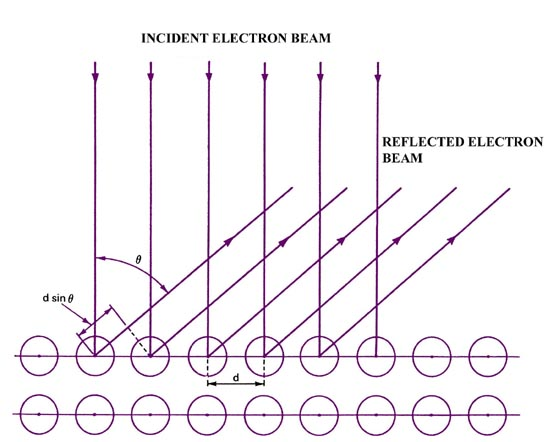
\includegraphics[width=8cm]{Duality/davisson.jpg}
\caption{电子在晶格上的衍射。}
%\label{default}
\end{center}
\end{figure}

假设电子由正上方垂直入射到镍晶体上,所谓晶体是原子的周期性排列,我们把每个原子都想象为一个障碍物,当电子如波一样撞到原子上时就和水波撞到芦苇上一样,我们可把障碍物看做是个新的波源,波撞在障碍物上然后向四面八方发射出去。

这时晶体上的每个格点都是一个新的波源,假设格点间的间距是$d$,或说假设晶格中存在着以$d$为周期的平移对称性,我们就可以构造如图一束束垂直入射,然后向某个方向$\theta $散射的电子波束。

我们考虑相邻的两列向$\theta$方向散射出去的波,然后计算它们之间的相位差。波动的相位和$(k x - \omega t)$有关,$t$是时间,对大家都一样,那么相位差就只和$x$有关。如图两列波走过的路程是不一样的,它们都由上方的无穷远入射,出射到$\theta$方向的无穷远去。

因此路程差是:

\begin{equation}
d \sin \theta 
\end{equation}

假设相邻两列波的路程差正好是一倍的波长:

\begin{equation}
d \sin \theta = \lambda
\end{equation}

或:

\begin{equation}
\theta =  \sin^{-1} \frac{\lambda }{d }
\end{equation}

我们将能观察到一个波峰遇波峰的情况,即相干地加强!如果物质波的波长$\lambda$和晶格的间距$d$差不多,我们会比较容易观察到这个波的加强。

假设不考虑电子的相对论效应,自由电子的能量是:

\begin{equation}
E = \frac{p^2}{2 m}
\end{equation}

电子的动量是:

\begin{equation}
p = \sqrt{ 2 m E  } = \frac{h }{\lambda }
\end{equation}

我们可估计出电子入射的能量:

\begin{equation}
E = \frac{ h^2 }{ 2 m \lambda^2 }
\end{equation}

计算出来的结果是$2.4 \times 10^{-17} $焦耳,或$150$电子伏。


\subsection*{练习}

\begin{enumerate}
\item 

在一个恒星系统中,行星离恒星越近它的温度就越高,反之则温度越低,我们可以针对特定恒星计算它的宜居带,即围绕恒星的带状区域,离恒星既不近也不远,温度正好处于$0-100 {}^o C$之间。

现在已知有这样一颗恒星Kepler-186(主序M1-型矮星),它的表面温度是3788开尔文,半径是0.47倍太阳半径,质量是0.48太阳质量。

求:(a)这颗星的颜色;(b)它的宜居带——即使行星表面温度处于$0-100 {}^o C$之间——距离恒星的最近和最远距离。


\item

由黑体辐射公式导出维恩位移定律:能量密度极大值所对应的波长$\lambda_m$与温度$T$成反比,即:$\lambda_m T = B$,$B$是一常量,近似计算$B$的数值。

解: 由频率的分布$\int u_T(\nu) d\nu$出发:

\begin{equation*}
\int u_T(\nu)d\nu =\int  \frac{8\pi h
\nu^3}{c^3}\frac{1}{e^{\frac{h\nu}{k_B T}} -1} d \nu
\end{equation*}

变量变换,把$\nu \to \lambda$, $\lambda = \frac{c}{\nu}$, $d \lambda = - \frac{c}{\nu^2} d \nu$. 或:$\nu = \frac{c}{\lambda}$, $d\nu = - \frac{\nu^2}{c} d\lambda=-\frac{c}{\lambda^2}d\lambda$。

\begin{equation*}
\int u_T(\nu) d \nu = \int \frac{8\pi
hc}{\lambda^5}\frac{1}{e^{\frac{hc}{k_B T\lambda}}-1} d\lambda
\end{equation*}

上式中我们把负号“-”略去不写. 现在对新的$\int u_T(\lambda)
d\lambda$中的$u_T(\lambda)$求微分. 极值条件:

\begin{equation*}
\left. {\frac{d u_T(\lambda)}{d\lambda}} \right|_{\lambda =
\lambda_{max}} = 0
\end{equation*}

令: $x = \frac{hc}{k_B T \lambda}$, 上式化简可得:

\begin{equation*}
(5-x)e^x =5
\end{equation*}

这个方程可通过``作图法''求解\footnote{Mathematica:
``FindRoot[5*Exp[x]-x*Exp[x] ==5 , \{x,10\}]''

``解析解'', 网址:

\url{http://www.udel.edu/physics/csaapt/Fall2002/files/analytic-solutions.doc}},

解出: $x \approx 4.97$, 即:

\begin{equation*}
\frac{hc}{k_B T \lambda_{max}} = 4.97
\end{equation*}

即:

\begin{equation*}
    \lambda_{max} T =\frac{hc}{4.97 k_B} = 2.898 \times 10^{-3} m \cdot K
\end{equation*}

值得注意的是如果我们由$\int u_T(\nu) d \nu$出发, 对$u_T(\nu)$求偏导, 即: $\left.{ \frac{d u_T(\nu)}{d \nu}} \right|_{\nu = \nu_{max}}= 0$, 所求出的$\nu_{max}$与$\lambda_{max}$不是一个“颜色”,即这样定义的$\lambda_{max} \nu_{max} \neq c$。

令$\frac{h\nu}{k_BT} = x $,由$\left.{ \frac{d u_T(\nu)}{d \nu}} \right|_{\nu = \nu_{max}}= 0$得到:

\begin{equation*}
    (3-x)e^x = 3
\end{equation*}

利用Mathematica中的FindRoot命令

\begin{verbatim}
    FindRoot[3*Exp[x]-x*Exp[x]==3, {x,10}]
\end{verbatim}

解出: $x \approx 2.82 $, 即:


\begin{equation*}
\frac{h\nu_{max}}{k_BT} = 2.82
\end{equation*}

\end{enumerate}


